La Figura \ref{fig:20230316200536} está formada por dos prismas rectangulares.
\textbf{Encuentra el volumen de la figura completa al sumar los volúmenes de las figuras separadas.}

\begin{minipage}{0.45\textwidth}
    \begin{figure}[H]
        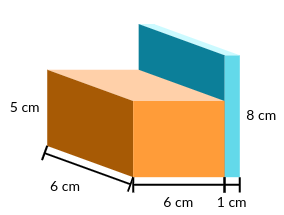
\includegraphics[width=0.9\linewidth]{../images/20230316200536}
        \caption{}
        \label{fig:20230316200536}
    \end{figure}
\end{minipage}
\begin{minipage}{0.45\linewidth}
    \begin{choices}
        \choice $(2 \text{cm} \times 7 \text{cm})+(1 \text{cm} \times 6 \text{cm} \times 8 \text{cm})$
        \choice $(2 \text{cm} \times 7 \text{cm} \times 1 \text{cm})+(1 \text{cm} \times 6 \text{cm} \times 8 \text{cm})$
        \CorrectChoice $(2 \text{cm} \times 8 \text{cm} \times 7 \text{cm})+(1 \text{cm} \times 6 \text{cm} \times 8 \text{cm})$
        \choice $(2 \text{cm} \times 7 \text{cm})+(8 \text{cm} \times 6 \text{cm})$
    \end{choices}
\end{minipage}
